\chapter{PRIMEIRA ITERAÇÃO}
\label{cap3}

A primeira iteração do algoritmo de inversão tem por objetivo a obtenção do gradiente de
velocidades em profundidade do modelo de velocidades de background, este resultado é oque
chamamos de primeira iteração. O modelo inicial utilizado é um modelo de velocidades homogêneo
e de velocidade constante igual a 1.5Km/s correspondente a velocidade próxima da superfície de aquisição. 

\begin{figure}[H]
\caption{Modelo de velocidade constante utilizado para a configuração inicial da
posição das fontes pontuais PIN (cruzes em preto).}
\begin{center}
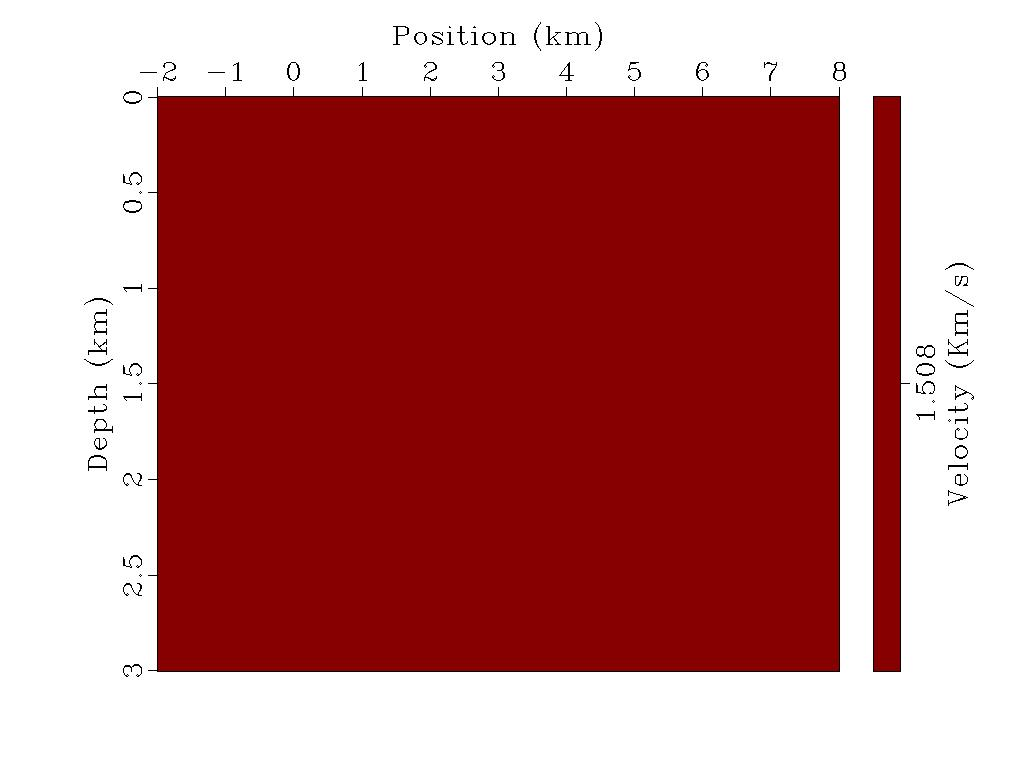
\includegraphics[scale=0.3]{images/ctevel.jpeg}
\vspace{-0.3cm}
\end{center}
\begin{center}
 Fonte: Do Autor.
\end{center}
\label{fig:3.1}
\end{figure}


Para a otimização do modelo de velocidades é utilizada a Equação \ref{eq:2.2} da soma das
diferenças nos tempos de trânsito obtidos com o tratamento de raios e os tempos de trânsito calculados utilizando a fórmula do ERC (Equação \ref{eq:2.1}). Nesta etapa, é utilizado o algoritmo Very Fast Simulated Annealing (VFSA) para realizar a otimização do gradiente de profundidade do modelo de velocidades. O modelo de velocidades é atualizado a cada iteração do algoritmo para cada valor do gradiente e segue a seguinte função de velocidades:

\begin{equation}
\label{eq:4.1}
v(z)=z g_z+v_0
\end{equation}

Em \ref{eq:4.1} a velocidade $v(z)$ cresce linearmente com a profundidade.

\begin{figure}[H]
\caption{Modelo obtido após a otimização do gradiente de velocidades em profundidade.
O valor do gradiente obtido após a otimização é $0.1673 s^-1$.}
\begin{center}
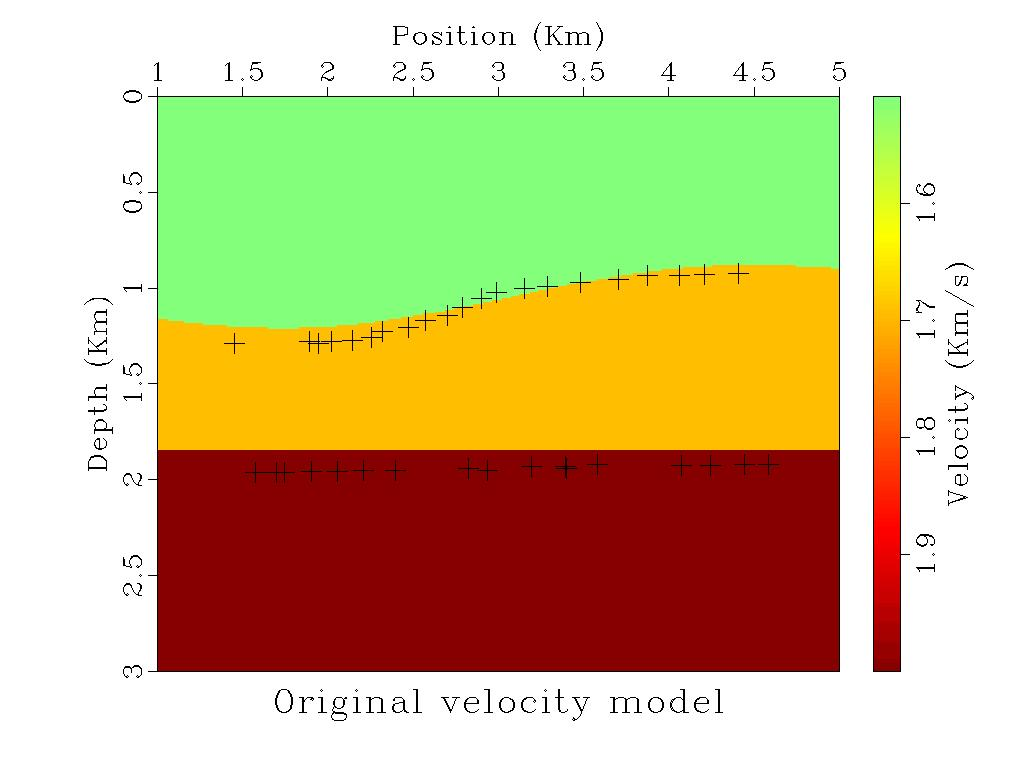
\includegraphics[scale=0.3]{images/gzvel.jpeg}
\vspace{-0.3cm}
\end{center}
\begin{center}
 Fonte: Do Autor.
\end{center}
\label{fig:3.2}
\end{figure}

\begin{figure}[H]
\caption{Modelo de velocidade constante e o modelo de velocidades com gradiente constante.
As cruzes em preto representam a localização das fontes PIN.}
\begin{center}
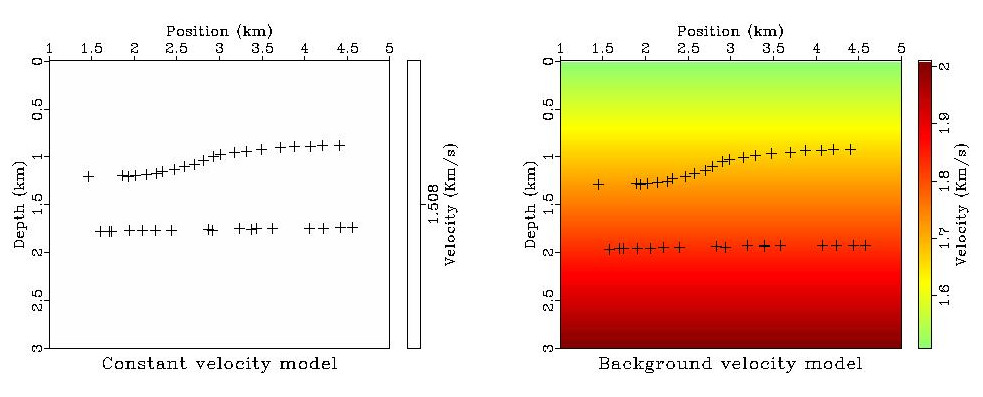
\includegraphics[scale=2]{images/compare.jpeg}
\vspace{-0.3cm}
\end{center}
\begin{center}
 Fonte: Do Autor.
\end{center}
\label{fig:3.3}
\end{figure}


O valor mínimo da diferença entre os tempos de trânsito (Equação \ref{eq:2.2}) será obtido para o gradiente de velocidades ótimo este valor é armazenado e utilizado para gerar o modelo de velocidades
da Figura \ref{fig:3.2}. Este modelo será o modelo de background utilizado na etapa da inversão.

\begin{figure}[H]
\caption{Localização das fontes PIN obtidas no modelo de velocidade constante
plotadas sobre o modelo de velocidades original (à esquerda)
e localização das fontes PIN obtidas no modelo de velocidades com gradiente constante
plotadas sobre o modelo de velocidades original (à direita).
As cruzes em preto representam a localização das fontes PIN.}
\begin{center}
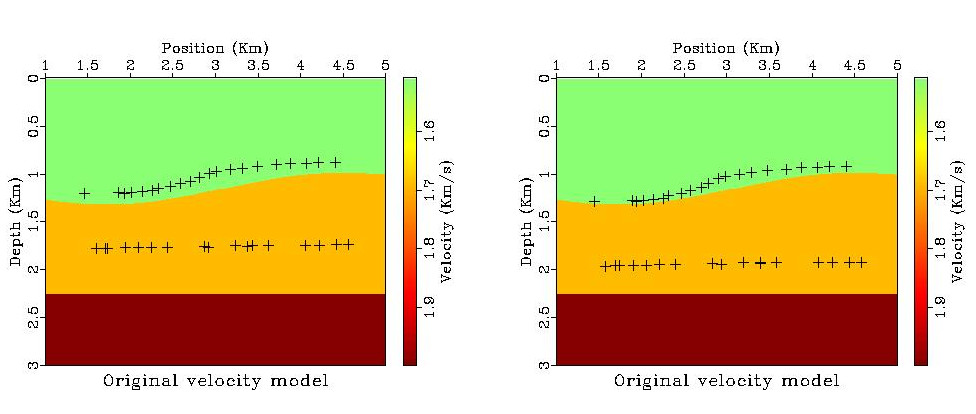
\includegraphics[scale=2]{images/resultinv.jpeg}
\vspace{-0.3cm}
\end{center}
\begin{center}
 Fonte: Do Autor.
\end{center}
\label{fig:3.4}
\end{figure}
